\documentclass[11pt, addpoints, answers]{exam}

\usepackage{amsmath, amssymb, euler}
\usepackage{xcolor}

% For inserting code snippets.
\usepackage{listings}
\lstset{
    columns = fixed,
    basewidth = {0.5em},
    breaklines = true,
    backgroundcolor = \color{white},
    keywordstyle = \color[RGB]{40, 40, 255},
    numberstyle = \footnotesize\color{darkgray},
    commentstyle = \ttfamily\color{violet},
    basicstyle = \ttfamily,
    stringstyle = \ttfamily\color[RGB]{128, 0, 0},
    showstringspaces = false,
    language = {[11]C++},
    escapechar = \@
}
\lstnewenvironment{cpp}[1][]{\lstset{language = {[11]C++}, #1}}{}

\usepackage{tikz}

% headers, footers, titles
\newcommand{\CourseName}{CS101 Algorithms and Data Structures}
\newcommand{\HomeworkNO}{Homework 3}
\newcommand{\DueDate}{Due date: 23:59, October 12th, 2022}

\pagestyle{headandfoot}
\runningheadrule
\runningheader{\CourseName}{\HomeworkNO}{\DueDate}
\runningfooter{}{\thepage}{}

\title{
	\CourseName\\
	Fall 2022\\
	\HomeworkNO
}
\author{}
\date{\DueDate}

% formats of questions, choices, points, etc.
\qformat{\bf\thequestion. (\totalpoints\ points) \thequestiontitle\hfill}
\pointname{'}
\CorrectChoiceEmphasis{\bf\color{blue}}

% We frequently use this font.
\newcommand{\ttt}{\texttt}

\begin{document}

\maketitle

\begin{enumerate}
	\item Please write your solutions in English.
	\item Submit your solutions to gradescope.com.
	\item Set your FULL name to your Chinese name and your STUDENT ID correctly in Account Settings.
	\item If you want to submit a handwritten version, scan it clearly. \ttt{CamScanner} is recommended.
	\item When submitting, match your solutions to the problems correctly.
	\item No late submission will be accepted.
	\item Violations to any of the above may result in zero points.
\end{enumerate}

\begin{questions}

\newpage

\titledquestion{Which Sort?}

Given a sequence
\[A=\langle 4,10,18,15,5,1,5,14,7,7\rangle,\]
we have performed some different sorting algorithms on it, during which some intermediate results are printed. Note that the steps you see below are \textbf{not} necessarily consecutive steps in the algorithm, but they are guaranteed to be in the correct order.

For each group of steps, guess (\(\surd\)) what the algorithm is. The algorithm might be one among the following choices:
\begin{itemize}
  \item Insertion-sort, implemented in the way that avoids swapping elements
  \item Bubble-sort, which stops immediately when no swap happens during one iteration
  \item Merge-sort
  \item Quick-sort, with pivot chosen to be \(A_l\) when partitioning a subarray \(A_l,\cdots,A_r\).
\end{itemize}

%%%%%%%%%%%%%%%%%%%%%%%%%%%%%%%%%%%%%%%%%%%%%%%%%%%%%%%%%%%%%%%%%%
% On the correct choice, replace `\choice' with `\CorrectChoice'.
%%%%%%%%%%%%%%%%%%%%%%%%%%%%%%%%%%%%%%%%%%%%%%%%%%%%%%%%%%%%%%%%%%

\begin{parts}
  \part[2]
  \[\begin{aligned}
    \langle 4,10,18,15,5,1,5,14,7,7\rangle,\\
    \langle 4,10,18,5,15,1,5,14,7,7\rangle,\\
    \langle 4,10,5,15,18,1,5,14,7,7\rangle,\\
    \langle 4,5,10,15,18,1,5,14,7,7\rangle.
  \end{aligned}\]
  \begin{oneparcheckboxes}
    \choice Insertion-sort
    \choice Bubble-sort
    \CorrectChoice Merge-sort
    \choice Quick-sort
  \end{oneparcheckboxes}
  
  \part[2]
  \[\begin{aligned}
    \langle 4,10,15,18,5,1,5,14,7,7\rangle,\\
    \langle 4,5,10,15,18,1,5,14,7,7\rangle,\\
    \langle 1,4,5,10,15,18,5,14,7,7\rangle,\\
    \langle 1,4,5,5,10,15,18,14,7,7\rangle.
  \end{aligned}\]
  \begin{oneparcheckboxes}
    \CorrectChoice Insertion-sort
    \choice Bubble-sort
    \choice Merge-sort
    \choice Quick-sort
  \end{oneparcheckboxes}

  \part[2]
  \[\begin{aligned}
    \langle 4,10,15,5,1,5,14,7,7,18\rangle,\\
    \langle 4,10,5,1,5,14,7,7,15,18\rangle,\\
    \langle 4,5,1,5,10,7,7,14,15,18\rangle,\\
    \langle 4,1,5,5,7,7,10,14,15,18\rangle.
  \end{aligned}\]
  \begin{oneparcheckboxes}
    \choice Insertion-sort
    \CorrectChoice Bubble-sort
    \choice Merge-sort
    \choice Quick-sort
  \end{oneparcheckboxes}

  \part[2]
  \[\begin{aligned}
    \langle 1,4,18,15,5,7,5,14,7,10\rangle,\\
    \langle 1,4,18,15,5,7,5,14,7,10\rangle,\\
    \langle 1,4,10,15,5,7,5,14,7,18\rangle,\\
    \langle 1,4,7,5,7,5,10,14,15,18\rangle.
  \end{aligned}\]
  \begin{oneparcheckboxes}
    \choice Insertion-sort
    \choice Bubble-sort
    \choice Merge-sort
    \CorrectChoice Quick-sort
  \end{oneparcheckboxes}
\end{parts}

\newpage

\titledquestion{Best Sort}

There is no such thing as a generally `best' sorting algorithm on all kinds of problems. For each of the following situations, choose (\(\surd\)) the most suitable sorting algorithm. Your choice should be the one that satisfies all the special constraints and is most efficient.

%%%%%%%%%%%%%%%%%%%%%%%%%%%%%%%%%%%%%%%%%%%%%%%%%%%%%%%%%%%%%%%%%%
% On the correct choice, replace `\choice' with `\CorrectChoice'.
%%%%%%%%%%%%%%%%%%%%%%%%%%%%%%%%%%%%%%%%%%%%%%%%%%%%%%%%%%%%%%%%%%

\begin{parts}
  \part[2] Sorting an array of coordinates of points \(\langle(x_1,y_1),\cdots,(x_n,y_n)\rangle\) on a 2d plane in ascending order of the \(x\) coordinate, while preserving the original order of the \(y\) coordinate for any pair of elements \((x_i,y_i),(x_j,y_j)\) with \(x_i=x_j\).

  \begin{oneparcheckboxes}
    \choice Insertion-sort
    \choice Bubble-sort
    \CorrectChoice Merge-sort
    \choice Quick-sort
  \end{oneparcheckboxes}

  \part[2] Sorting an array that is \emph{almost} sorted with only \(n/2\) inversions due to some kind of perturbation.

  \begin{oneparcheckboxes}
    \CorrectChoice Insertion-sort
    \choice Bubble-sort
    \choice Merge-sort
    \choice Quick-sort
  \end{oneparcheckboxes}

  \part[2] Sorting an array on an embedded system with quite limited memory. You may only use \(\Theta(1)\) extra space, but a higher time cost is acceptable.

  \begin{oneparcheckboxes}
    \CorrectChoice Insertion-sort
    \choice Quick-sort
    \choice Merge-sort
  \end{oneparcheckboxes}
\end{parts}

\newpage

\titledquestion{Multiple Choices}

Each question has \textbf{one or more} correct answer(s). Select all the correct answer(s). For each question, you will get 0 points if you select one or more wrong answers, but you will get 1 point if you select a non-empty subset of the correct answers.

Write your answers in the following table.

%%%%%%%%%%%%%%%%%%%%%%%%%%%%%%%%%%%%%%%%%%%%%%%%%%%%%%%%%%%%%%%%%%%%%%%%%%%
% Note: The `LaTeX' way to answer a multiple-choices question is to replace `\choice'
% with `\choice', as what you did in the previous questions. However, there are 
% still many students who would like to handwrite their homework. To make TA's work 
% easier, you have to fill your selected choices in the table below, no matter whether 
% you use LaTeX or not.
%%%%%%%%%%%%%%%%%%%%%%%%%%%%%%%%%%%%%%%%%%%%%%%%%%%%%%%%%%%%%%%%%%%%%%%%%%%

\begin{table}[htbp]
	\centering
	\begin{tabular}{|p{1.7cm}|p{1.7cm}|p{1.7cm}|p{1.7cm}|p{1.7cm}|p{1.7cm}|p{1.7cm}|p{1.7cm}|p{1.7cm}|}
		\hline
		(a) & (b) & (c) & (d) & (e) & (f) \\
		\hline
		%%%%%%%%%%%%%%%%%%%%%%%%%%%%%%%%%%%%%%%%%%%%%%%%%%%%%%%%%%
		% YOUR ANSWER HERE.
		    &     &     &     &     &     \\
		%%%%%%%%%%%%%%%%%%%%%%%%%%%%%%%%%%%%%%%%%%%%%%%%%%%%%%%%%%
		\hline
	\end{tabular}
\end{table}

\begin{parts}
    \part[2] A planar graph is a graph which can be embedded in a plane i.e. you can find a way to put all vertices on the plane where the edges will not intersect with each other. Which of the statement(s) is/are correct?
    \begin{choices}
        \choice $\forall n\leq 5, K_n$ is planar. $K_n$ means the complete graph with $n$ vertices.
        \choice $K_6$ is not planar.
        \choice DAGs are planar.
        \choice A tree is planar.
        \choice Bipartite graphs are planar.
    \end{choices}

    \part[2] Given a graph $G=(V,E)$, $w(e)$ indicates the weight of edge $e$. Which of the statement(s) is/are correct?
    \begin{choices}
        \choice Both Kruskal's and Prim's algorithms can correctly find the MST even when $\exists e, w(e)<0$.
        \choice Suppose $G$ is connected and $|E| = \omega(|V|)$, $G$ has a unique MST if and only if $\forall e,e'\in E, w(e) = w(e') \Leftrightarrow e = e'$ i.e. weights of edges are distinct.
        \choice Suppose $G' = (V,E)$ is the same graph as $G$ with different weight function $v(e)$. If they share a same MST $T$, then $T$ is also the MST of $G$ with weights $u(e) = w(e) + v(e)$.
        \choice If $G$ contains multi-edges i.e. $G$ is not simple, then Kruskal's algorithm will fail but Prim's won't fail when finding MST.
    \end{choices}

	\part[2] Given a graph $G=(V,E)$, which of the following is(are) correct? 
	\begin{choices}
		\choice If $G$ is a complete graph with $4$ vertices, then the number of spanning trees of $G$ is $16$.
		\choice After Kruskal's algorithm, we choose $m$ edges, then the number of connected components of $G$ is $|V|-m$.
		\choice If $G$ is stored in adjacency matrix, then the total time complexity of Kruskal's algorithm can reach $\Theta(|V|^2+|E|\log|E|)$.
        \choice Suppose $G$ is connected and $|V| = |E|$, the maximum number of spanning trees of $G$ can reach $\Theta(|V|)$.
	\end{choices}
    
    \part[2] Let $G$ be a weighted undirected graph with positive weights where edge $e$ has weight $w_e\in \mathbb{R}^+$ for all $e \in E$. A new graph $G'$, which is a copy of $G$, and the weight of each edge $e$ in $G'$ is transformed using a function $f(w_e)$. Which of the following statements is/are true?

    \begin{choices} 
        \choice If $f(w_e) = w_e^2$, then any MST in $G$ is also an MST in $G'$.
        \choice If $f(w_e) = 2^{w_e}$, then any MST in $G$ is also an MST in $G'$.
        \choice If $f(w_e) = \frac1 {w_e}$, then any MST in $G$ is also an MST in $G'$.
        \choice If $f(w_e) = \log (w_e)$, then any MST in $G$ is also an MST in $G'$.
    \end{choices}

	\part[2] What is the number of spanning trees of following graph?

    \begin{center}
    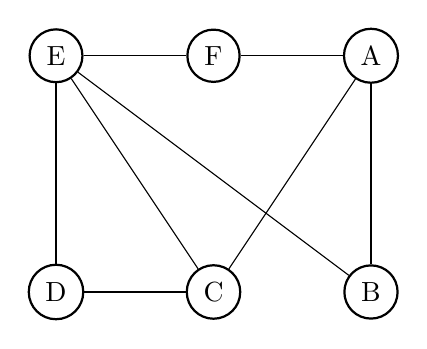
\begin{tikzpicture}
        \begin{scope}[every node/.style = {circle, thick, draw}]
            \node (A) at (2,0) {A};
            \node (B) at (2, -3) {B};
            \node (C) at (0, -3) {C};
            \node (D) at (-2, -3) {D};
            \node (E) at (-2, 0) {E};
            \node (F) at (0,0) {F};
        \end{scope}
        \begin{scope}
            \path[-] (E) edge (D);
            \path[-] (E) edge (C);
            \path[-] (E) edge (B);
            \path[-] (C) edge (D);
            \path[-] (B) edge (A);
            \path[-] (A) edge (C);
            \path[-] (A) edge (F);
            \path[-] (E) edge (F);
        \end{scope}
    \end{tikzpicture}
    \end{center}
	\begin{choices}
		\choice 32
		\choice 34
		\choice 36
		\choice 38
	\end{choices}

        \part[2] Which of the following statements are true for MST(Minimum Spanning Tree)?
        \begin{choices}
            \choice Suppose $G$ has multiple MSTs. For each minimum spanning tree $T$ of a graph $G$, there is a way to sort the edges of $G$ in Kruskal’s algorithm so that the algorithm returns $T$.
            \choice Prim's algorithm is a divide-and-conquer algorithm because it divides the graph into $S$ and $V-S$ then solve.
            \choice If we use binary heap to optimize Prim's algorithm when choosing the next edge, it will always have a better time complexity than the original algorithm on any graph.
            \choice If we add a new edge $e = (u,v)$ into a graph $G=(V,E)$ with unique MST to get a new graph $G' = (V,E\cup\{e\})$. There is at most $1$ edge difference between the MST of $G$ and $G'$.
        \end{choices}

\end{parts}


\newpage

\titledquestion{New $k$-th Minimal Value}

Given two \textbf{sorted} arrays $\langle a_1,\cdots,a_n\rangle$ of length $n$ and $\langle b_1,\cdots,b_m\rangle$ of length $m$ with $n + m$ \textbf{distinct} elements and an integer $k$ ($1 \le k \le n + m$), we will design a \textbf{divide and conquer} algorithm to find $k$-th minimal element in the merged array $\langle a_1,\cdots,a_n, b_1, \cdots, b_m\rangle$ of length $n + m$. We say $a_x$ is the $k$-th minimal value of $a$ if there are exactly $k-1$ elements in $a$ that are less than $a_x$, i.e.
\[\left|\left\{i\mid a_i<a_x\right\}\right|=k-1.\]

\begin{parts}
    \part[6] You should design a \textbf{divide and conquer} algorithm with time complexity $O(\log n + \log m)$.
    \begin{solution}
        %%%%%%%%%%%%%%%%%%%%%%%%%%%%%%%%%%%%%%%%%%%%%%%%%
        % Replace `\vspace{2in}' with your answer.
        we do binary search for two arrays together
        
        let mida,midb be the middle point of array a,b

        and we take out two subarray a', b' from array a,b
      
        start at their left bound, end at their middle,and mark the subarray's size be la,lb

        without loss of generality, we regard a'[mida] < b'[midb].(if opposite, we just need to swap the two array and do it again)

        and we need to discuss:

        if $l1+l2\leq k$,then all of the elements in a' must have the index $\leq k$ in the merged array,so we take them and solve the subproblem.

        if $l1+l2 > k$,then all of the elements in b but not in b' must not have the index $\leq k$ in the merged array,so we do not take them, and solve the subproblem
        \paragraph{Algorithm Design:} 
        we do binary search for two arrays together
        \begin{enumerate}
          \item get the middle point mida, midb of array a,b 
          \item compare a[mida] and b[midb], to make sure that a have the less element, if not, just swap the two arrays and do it again
          \item compare $l1+l2$ and $k$, and solve the subproblem we discussed above
        \end{enumerate}

        \paragraph{Pseudocode :}
        the lefta, righta is the left,right bound of array a in this subproblem,

        the leftb, rightb is the left,right bound of array b in this subproblem,

        $k$ means that we need to find the kth minimal element in the subprolem.

        $mida,midb$ are the middle point of the arrays

        l1,l2 are the length of the subarray that start at left bound and end at the middle
        \begin{algorithm}[H]
          \begin{algorithmic}[1]
            \Function {kth\_min}{$a$, $b$, $lefta$, $righta$, $leftb$, $rightb$, $k$}
            \If {$righta < lefta$} 
            \State \Return b[leftb+k-1]
            \EndIf
            \If {$rightb < leftb$} 
            \State \Return a[lefta+k-1]
            \EndIf
            \State $mida\gets (righta+lefta)/2$
            \State $midb\gets (rightb+leftb)/2$
            \If {$a[mida] > b[midb]$} 
            \State \Return kth\_min($b$, $a$, $leftb$, $rightb$, $lefta$, $righta$, $k$)
            \EndIf
            \State $l1\gets mida-lefta+1$
            \State $l2\gets midb-leftb+1$
            \If {$l1+l2 \leq k$} 
            \State \Return kth\_min($a$, $b$, $mida+1$, $righta$, $leftb$, $rightb$, $k-l1$)
            \Else
            \State \Return kth\_min($a$, $b$, $lefta$, $righta$, $leftb$, $midb-1$, $k$) 
            \EndIf   		
            \EndFunction
          \end{algorithmic}
        \end{algorithm}

        \paragraph{Time Complexity Analysis:}
        During each recursion, the calculation of 
        
        $mida,midb,l1,l2$ and comparison can be done in constant time, which is $O(1)$. 
        We ignore half of the elements after each comparison, thus we need $O(\log n)$ recursions for each array.
        and we have two arrays with length of n and m, so the complexity is to sum them usepackage

        which means that the complexity is $O(log n + log m)$.
        %\vspace{2.5in}
        %%%%%%%%%%%%%%%%%%%%%%%%%%%%%%%%%%%%%%%%%%%%%%%%%
      \end{solution}
    \part[6] You should design \textbf{another divide and conquer} algorithm with better time complexity $O(\log k)$. 
    \begin{solution}
      %%%%%%%%%%%%%%%%%%%%%%%%%%%%%%%%%%%%%%%%%%%%%%%%%
      % Replace `\vspace{2in}' with your answer.
      to shortly explain, in each subprolem, we need to take the first few elements from the remaining elements of array a and b, mark the new subarray we take out as a' and b'

      since a' and b' are sorted and have distincy elements,so we need to compare the last element of each new array,

      the new subarray with the shorter last element must all be involed in the first k element of the merged array, 

      so we need to delete them before solving the subproblem,

      as for the new subarray with the larger last element, we cannot make sure how many elements are in the merged array, so we just remain them, and figure out in the subproblem.
      \paragraph{Algorithm Design:} 
      we divide and conquer by using the half of the $k$
      \begin{enumerate}
          \item we get the value of $len=\lfloor \frac{k}{2} \rfloor$
          \item then we need to pick one element from each array, mark as a\_pick,b\_pick.
          which means that we are going to take the sequence from $pos$ to $pick$.(pos will be explained in the pseudo code part)
          \item to make it easier to write, we just let array a has less remaining elements.(if opposite, just swap the two arrays)
          \item if the length of the remaining elements of the array a $<len$, we just take the end of the element as pick.
          But we need to make sure that the sum of elements we take from array a and b should be $k$.
          \item then compare the element at a\_pick in a and at b\_pick in b.
          \item delete the elements from the array that is the less one from the result above, and let 
          $k\_new= k$ - (the number of elements we removed), and repeat the above operations until $k=1$ or one of the array is empty.
        
        
        \end{enumerate}

        \paragraph{Pseudocode:}
        $posa$ and $posb$ are indecies of the leftmost that still remain in given array $a,b$ respectively.
        
        $len(\cdot)$ is the function the get the array's size.
        And we set the index of the elements in array start at $1$
        
        to easier get the element that we need to compare, just let the array a be the short one,
        so we just need to add a judge that is the remaining of array a is less than b, then swap them.(the 2nd to 4th row of the pseudo code)
        then the array a always has less remain elements.
        
        \begin{algorithm}[H]
          \begin{algorithmic}[1]
            \Function {$kth\_min$}{$a$, $b$, $posa$, $posb$, $k$}
            \If {$(len(a)-posa+1) > (len(b)-posb+1)$} 
            \State \Return $kth\_min$($b$, $a$, $posb$, $posa$, $k$)
            \EndIf
            \If {$posa > len(a)$} 
            \State \Return b[posb+k-1]
            \EndIf
            \If {$posb > len(b)$} 
            \State \Return a[posa+k-1]
            \EndIf
            \If {$k==1$} 
            \State \Return max\{a[posa],b[posb]\}
            \EndIf
            \State $length\gets \lfloor k/2 \rfloor$
            \State $a\_remain\gets (len(a)-posa+1)$
            \If {$a\_remain<=length$}
            \State new\_posa=len(a)
            \Else
            \State new\_posa=(posa+length-1)
            \EndIf
            \State $new\_posb\gets(posb+k-(posa-new\_posa+1)-1)$
            \If {$a[new\_posa] < b[new\_posb]$} 
            \State \Return $kth\_min$($a$, $b$, $new\_posa+1$, $posb$, $k-(new\_posa-posa+1)$) 		
            \Else
            \State \Return $kth\_min$($a$, $b$, $posa$, $new\_posb+1$, $k-(new\_posb-posb+1)$) 		
            \EndIf
            \EndFunction
          \end{algorithmic}
        \end{algorithm}

        \paragraph{Time Complexity Analysis:}
        During each recursion, the calculation of
        
        $length,new\_posa,new\_posb$ and comparison can be done in constant time, which is $O(1)$. 
        after one recursion, the k become $\frac{k}{2}$ unless the short array turn to the end, but in that case, the function will finish,so
      
        $T(k) = T(\frac{k}{2})+O(1)$
        Therefore, by the Master Theorem $a=1,b=1,d=0,\log_{b}{a}=0=d$, so $T(k) = O(\log k)$.
      %\vspace{2.5in}
      %%%%%%%%%%%%%%%%%%%%%%%%%%%%%%%%%%%%%%%%%%%%%%%%%
    \end{solution}
  \end{parts}

\newpage

\titledquestion{Discovery}

\begin{parts}
  \part[2] Is C++ STL \lstinline{std::sort} stable or not? If not, is there any stable sort function provided by the standard library?
  \begin{solution}
    %%%%%%%%%%%%%%%%%%%%%%%%%%%%%%%%%%%%%%%%%%%%%%%%%
    % Replace `\vspace{0.5in}' with your answer.
    %\vspace{0.5in}
    \(C++ \ STL \ std::sort\) is not stable.

    but the \(std::stable\_sort\) is stable.

    %%%%%%%%%%%%%%%%%%%%%%%%%%%%%%%%%%%%%%%%%%%%%%%%%
  \end{solution}
  \part[0] Suppose \(A\) is an array of size \(n\). If we can find the median value of \(A\) within \(O(n)\) time, it is possible to make quick-sort \(\Theta(n\log n)\) in worst case. STFW (Search The Friendly Web) about how to find the median value in \(O(n)\) time.
  
  \begin{solution}
    %%%%%%%%%%%%%%%%%%%%%%%%%%%%%%%%%%%%%%%%%%%%%%%
    
    In the book \(Introduction oto algorithms\), and by searching the friendly internet, I found an algorithm
    called \(BFPRT\), the name is from five of its inventors.

    the algorithm is mainly decided by the following steps.
    
    \begin{itemize}
      \item divide the array into groups every five adjacent numbers
      \item for each group of numbers, we find the median of the five numbers and form a median array of the median of all groups
      \item the median of each group forms a new array
      \item recursively do the above steps
      \item finally there reamin only one number, the medium number of the whole array.
      
    \end{itemize}
    
    \(T(n) \leq  T(\frac{n}{5}) +T(\frac{7n}{10})+c \cdot n\)

    and it is proved on book and internet that \(T(n) \leq 10c \cdot n\)

    so \(T(n)=\Theta(n)\)
    
    actually, when I was learning algorithms before, I hearded that we can use stl in C++, the \(std::nth\_element(...)\) can find the 
    \(k\_th\) minimal element with in \(\Theta(n)\) time.

    the median element can be easily find by using it, so I just want to write it before scearching

    However, when I scearch the code of it clearly, I thought, and some analysis on the internet also 
    say that the time complexity of \(std::nth_element\) is \(\Theta(n)\) on average, instead of the worst case,
    the worst case might turn into \(\Theta(n^2)\)

    so it might not be the best way to find the medium number, the \(DFPRT\) algorithm can get the median in \(\Theta(n)\)
    %%%%%%%%%%%%%%%%%%%%%%%%%%%%%%%%%%%%%%%%%%%%%%%
  \end{solution}
  
  \part[0] It is known that some sorting algorithms, like quick-sort, need to swap elements. Run the following code, change the value of \(n\) and see how the output changes.
  \begin{cpp}
    #include <algorithm>
    #include <cstdlib>
    #include <iostream>
    #include <vector>

    namespace std {
      template <>
      inline void swap<int>(int &lhs, int &rhs) noexcept {
        auto tmp = lhs;
        lhs = rhs;
        rhs = tmp;
        std::cout << "swap is called.\n";
      }
    } // namespace std

    int main() {
      std::srand(19260817);
      constexpr int n = 10;
      std::vector<int> vec;
      for (auto i = 0; i != n; ++i)
        vec.push_back(std::rand());
      std::sort(vec.begin(), vec.end());
      return 0;
    }
  \end{cpp}
  From your observation, the \lstinline{swap} function is never called when \(n\leqslant\) \fillin[][2em]. What algorithm(s) does \lstinline{std::sort} use?
  \begin{solution}
    %%%%%%%%%%%%%%%%%%%%%%%%%%%%%%%%%%%%%%%%%%%%%%%
    % Replace `\vspace{0.7in}' with your answer.
    %\vspace{0.7in}
    the \lstinline{swap} function is never called when \(n\leqslant 16\) .

    the std::sort is based on the introspective sorting. It is combined with many different type
    of sorting algorithms, and it will execute different onces if it reach some different situations.

    the threshold of the std::sort is 16.

    \begin{itemize}
      \item the length of the array need to be sorted is less than or equal to the threshold
      the std::sort will execute the insertion-sort.
      
      \item the length of the array need to be sorted is more than the threshold,
        
      there is another value \(depth\_limit\), which usually set as \(2*logN\), N is the length of the array need to be sorted

      \begin{itemize}
        \item the time of the recursion is less than or equal to the \(depth\_limit\)
        
        it will execute the recursive quick-sort.

        \item the time of the recursion more than the \(depth \_ limit\)
        
        it will execute heap-sort.
      \end{itemize}

    \end{itemize}
     

    %%%%%%%%%%%%%%%%%%%%%%%%%%%%%%%%%%%%%%%%%%%%%%%
  \end{solution}
\end{parts}

\end{questions}

\end{document}